\chapter{Estado del Arte}\label{chapter:state-of-the-art}


\colorbox{lightgray}{\textbf{//TODO: Presentacion del capitulo: qué se va a tratar y por qué}}

\section{Qué es una Blockchain}
En esencia, una blockchain es un \textbf{\textit{ledger}} distribuido que registra todas las transacciones que tienen lugar en la red. El \textit{ledger} de una \textit{blockchain} a menudo se describe como descentralizado porque se replica entre muchos participantes de la red, cada uno de los cuales colabora en su mantenimiento.

La información registrada en una \textit{blockchain}, además de ser \textbf{descentralizada} y \textbf{colaborativa}, sólo se puede agregar. Esto significa que se garantiza, utilizando técnicas criptográficas, que una vez  agregada una transacción al \textit{ledger}, no se puede modificar. Esta propiedad de inmutabilidad simplifica la determinación de la procedencia de la información pues los participantes pueden estar seguros de que esta no ha cambiado después de añadirse a la \textit{blockchain}.

Con el fin de respaldar la actualización constante de la información, y  habilitar una gran cantidad de funciones del \textit{ledger} (transacciones, consultas, etc.), una red  blockchain utiliza \textbf{contratos inteligentes}. Estos constituyen una forma de proporcionar acceso controlado al \textit{ledger}.

Una red  \textit{blockchain} se compone principalmente de un conjunto de \textbf{nodos \textit{peers}} (o simplemente \textit{peers}). Dichos nodos son un elemento fundamental de la red debido a que alojan \textit{ledgers} y contratos inteligentes.

Se le llama \textbf{consenso} al proceso de mantener las transacciones sincronizadas a través de la red con el objetivo de garantizar que los \textit{ledgers} se actualicen solo cuando las transacciones sean aprobadas por los participantes apropiados; y con las transacciones en el mismo orden.

\section{Hyperledger Fabric}

Hyperledger Fabric, o simplemente Fabric, es uno de los proyectos de blockchain dentro de Hyperledger [\cite{hyperledger-foundation}], auspiciado por la Fundación Linux [\cite{linux-foundation}]. Es una plataforma de \textbf{tecnología de \textit{ledger} distribuido} (DLT por sus siglas en inglés) de código abierto, diseñada para su uso en contextos empresariales. Además, se define como una red permisionada, lo que significa que los participantes se conocen entre sí, en lugar de ser anónimos. 

Al igual que otras tecnologías \textit{blockchain}, Hyperledger Fabric cuenta con un \textit{\textbf{ledger}}, utiliza \textbf{contratos inteligentes} y es un sistema mediante el cual los participantes realizan sus \textbf{transacciones}.

Las redes de Hyperledger Fabric son administradas por una colección de \textbf{organizaciones}. Los nodos \textit{\textbf{peer}} son fundamentales para construir este tipo de red distribuida porque son propiedad de estas organizaciones y sus puntos de conexión a la red. 

Al ser una plataforma permisionada, Hyperledger Fabric permite la confidencialidad a través \textbf{canales}. En estos, los participantes establecen una \textit{sub-red} donde cada miembro tiene visibilidad de un conjunto particular de transacciones. Así, solo aquellos nodos que participan en un canal tienen acceso al contrato inteligente y a los datos transados, preservando la privacidad y confidencialidad de ambos.
Esta es una opción especialmente importante para las redes en las que algunos participantes pueden ser competidores y no quieren que cada transacción sea conocida por el resto de la red. 

%Fabric es la primera plataforma DLT que admite \textbf{contratos inteligentes} creados en lenguajes de programación de propósito general como Java, Go y Node.js, en lugar de lenguajes específicos de dominio restringidos (DSL).

\subsection*{Ledger}

El \textit{ledger} de Hyperledger Fabric consta de dos componentes: el \textbf{world state} y el \textbf{registro de transacciones}. Cada participante tiene una copia del \textit{ledger} de cada red de Hyperledger Fabric a la que pertenece.

El componente de \textit{world state} describe el estado del \textit{ledger} en un momento determinado, es la base de datos del mismo. El componente de registro de transacciones almacena todas las transacciones que dieron como resultado el valor actual del \textit{world state}. Es el historial de actualizaciones del \textit{world state}. El \textit{ledger}, entonces, es una combinación de la base de datos del \textit{world state} y el historial del registro de transacciones.

\subsection*{Contratos inteligentes}

Los desarrolladores de aplicaciones de cada organización pueden crear \textbf{contratos inteligentes }para implementar un proceso comercial compartido por los miembros del consorcio. Los contratos inteligentes se utilizan para ayudar a generar \textbf{transacciones} que luego se pueden distribuir a cada nodo de la red.

Los contratos inteligentes de Hyperledger Fabric se definen dentro del \textbf{\textit{chaincode}}. Se pueden definir múltiples contratos inteligentes dentro del mismo \textit{chaincode}. Cuando este despliega, todos los contratos inteligentes dentro de él se hacen disponibles para las aplicaciones externas a la \textit{blockchain}. Una aplicación  invoca al contrato inteligente cuando esta necesita interactuar con el \textit{ledger}. 

En la mayoría de los casos, el \textit{chaincode} interactúa sólo con el componente de la base de datos del ledger, el \textbf{\textit{world state}} (consultándolo, por ejemplo) y no con el registro de transacciones.

Los usuarios de Hyperledger Fabric a menudo usan los términos \textbf{contrato inteligente} y \textbf{\textit{chaincode}} indistintamente. En general, un contrato inteligente define la lógica de transacción que controla el ciclo de vida de un objeto contenido en el \textit{world state}; luego, este se empaqueta en un \textit{chaincode} para desplegarse a una red \textit{blockchain}.

\subsection*{Consenso}
Las transacciones deben escribirse en el ledger en el orden en que ocurren, aunque puedan ser entre diferentes conjuntos de participantes dentro de la red. Para que esto suceda, se debe establecer el orden de las transacciones y se debe implementar un método para rechazar transacciones incorrectas que se hayan insertado en el ledger por error (o maliciosamente).

Los \textit{peers} ejecutan un \textbf{protocolo de consenso} que abarca desde la propuesta y la aprobación de transacciones hasta el orden, la validación y el despliegue de las mismas a través de la red.
En pocas palabras, el \textbf{consenso} se define como la verificación completa de la correctitud de un conjunto de transacciones que componen un bloque [\cite{hlf-doc}].

El consenso está mediado por nodos especiales llamados \textit{\textbf{orderers}}, encargados de ordenar las transacciones. Un conjunto de nodos \textit{orderers} forman un \textbf{\textit{ordering service}}. Además de su rol de ordenar, estos nodos también mantienen la lista de organizaciones que pueden crear canales. Esta lista se conoce como el \textbf{consorcio}.

%Sin embargo, el consenso abarca más que simplemente acordar el orden de las transacciones, y esta diferenciación se destaca en Hyperledger Fabric a través de su papel fundamental en todo el flujo de transacciones, desde la propuesta y el respaldo hasta el pedido, la validación y el compromiso. 

\begin{figure}[tbph]
\centering
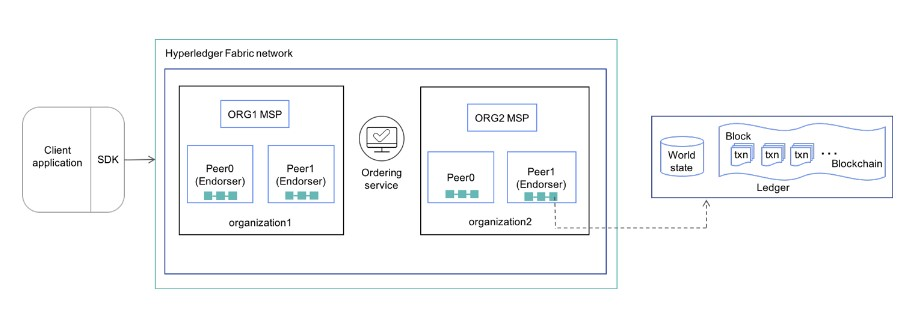
\includegraphics[width=\textwidth]{Images/hlf_components}
\caption{Componentes de Hyperledger Fabric}
\label{fig:hlfcomponents}
\end{figure}


\subsection*{Arquitectura para las transacciones \textit{execute-order-validate}.}

Fabric admite el uso de lenguajes de programación estándar en sus contratos inteligentes. Esto gracias a que implementa la arquitectura de ejecución de transacciones \textit{execute-order-validate}.

%Para entender por qué es posible añadir $C\sharp$ a la lista de lenguajes soportados por Hyperledger Fabric para programar contratos inteligentes, se dedicará esta sección a explicar dicha arquitectura.

Todos los sistemas de blockchains anteriores a Hyperledger Fabric, autorizados o no, siguen la arquitectura de ejecución de transacciones \textit{order-execute} [\cite{hlf-paper}]. Esto significa que la red blockchain ordena las transacciones primero, utilizando un protocolo de consenso, y luego los ejecuta en el mismo orden en todos los nodos \textit{peer} secuencialmente.

%La arquitectura \textit{order-execute} es conceptualmente simple y por lo tanto también muy utilizada. Sin embargo, tiene varios inconvenientes cuando se implementa en una blockchain autorizada de uso general.

Un problema importante para una arquitectura \textit{order-execute} son las transacciones no deterministas. Las operaciones que se ejecutan después del consenso deben ser deterministas, o el \textit{ledger} distribuido se “bifurca” y viola la premisa básica de una blockchain, que todos los nodos \textit{peer} tienen el mismo estado. Esto generalmente se aborda mediante la programación de \textit{blockchains} en un DSL (ej. Ethereum Solidity) que son lo suficientemente expresivos para sus aplicaciones pero limitados a una ejecución determinista.

Dichos lenguajes son difíciles de diseñar y requieren
aprendizaje adicional por parte del programador. La redacción de contratos inteligentes en un lenguaje de propósito general (p. ej., Go, Java, C/C++) parece más atractivo y acelera la adopción de soluciones blockchain.

%Desafortunadamente, los lenguajes de propósito general plantean muchos problemas para garantizar una ejecución determinista. Incluso si el desarrollador de la aplicación no introduce operaciones obviamente no deterministas, detalles ocultos de implementación pueden tener el mismo efecto devastador (por ejemplo, un
%iterador de mapa no es determinista en Go).

Fabric introduce la arquitectura de ejecución de transacciones \textit{order-execute-validate} y no sigue el diseño \textit{order-execute} estándar. Aborda los desafíos de resiliencia, flexibilidad, escalabilidad, rendimiento y confidencialidad que enfrenta el modelo \textit{order-execute} al separar el flujo de transacciones en tres pasos:
\begin{enumerate}
 \item \textbf{ejecutar} una transacción y verificar su correctitud, avalándola.
 \item \textbf{ordenar} transacciones a través de un protocolo de consenso.
   \item \textbf{validar} transacciones contra una política de aprobación específica de la aplicación antes de actualizar el \textit{ledger}.
\end{enumerate}

Este diseño se aparta del paradigma \textit{order-execute} en el sentido de que Fabric ejecuta transacciones antes de llegar a un acuerdo final sobre su orden. De esta forma se elimina cualquier no determinismo, ya que los resultados inconsistentes se pueden filtrar antes de ordenar.

Al eliminar el no determinismo, Fabric es la primera blockchain que permite el uso de lenguajes de programación estándar. 

%Gracias a esta posibilidad, en este trabajo se pretende añadir $C\sharp$ a la lista de lenguajes actualmente soportados.

%\subsection*{Flujo de una transacción}
%El flujo de solicitud de alto nivel de una transacción en una red de Hyperledger Fabric es así:
%
%\begin{enumerate}
%\item El cliente se conecta a una red de Hyperledger Fabric mediante Node.js o Java™ SDK. Usando la API SDK, el cliente crea una transacción y la envía al par que la respalda.
%
%\item El par que respalda verifica la firma del cliente, simula una transacción y envía una firma de respaldo.
%
%\item Si la transacción está endosada, el cliente envía la transacción al servicio de pedidos. De lo contrario, la transacción se cancela.
%
%\item El servicio de pedidos entrega una transacción a los pares. Todos los pares comprometen y aplican la misma secuencia de transacciones y actualizan su estado.
%\end{enumerate}

\begin{figure}[tbph]
\centering
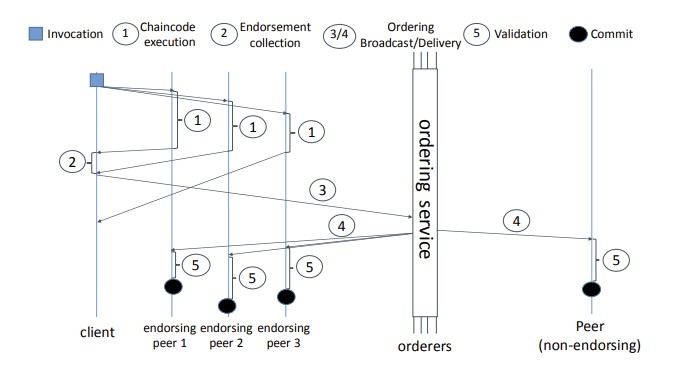
\includegraphics[width=\textwidth]{Images/transaction_flow}
\caption{Flujo de una transacción}
\label{fig:transactionflow}
\end{figure}



%Los lenguajes actualmente soportados son Java, Go y Node.js.
%Para entender cómo es posible añadir otro lenguaje para implementar contratos inteligentes, se hará énfasis en la fase de ejecución, donde el chaincode y el nodo peer se comunican. 

%\section{Fase de ejecución}
%
%En la fase de ejecución, los clientes firman y envían la propuesta de transacción a uno o más nodos \textit{peers} para su ejecución.  La propuesta es una solicitud para invocar una función del \textit{chaincode} con ciertos parámetros de entrada, con la intención de leer y/o actualizar el \textit{ledger}. Una aplicación que aprovecha un SDK compatible (Node, Java, Go) utiliza una de las API disponibles para generar una propuesta de transacción.
%
%El SDK sirve como un \textit{shim} para empaquetar la propuesta de transacción en el formato diseñado correctamente (\textit{protocol buffer} sobre gRPC) y toma las credenciales criptográficas del usuario para producir una firma única para esta propuesta de transacción. 



\section{fabric-contract-apis y fabric-chaincode-apis}
Hyperledger Fabric ofrece una serie de APIs para respaldar el desarrollo de contratos inteligentes (\textit{chaincode}) en varios lenguajes de programación (Go, Java y Node.js). 

Las \textit{fabric-chaincode-apis} son responsables de ejecutar el contrato inteligente, hacerlo accesible para el nodo \textit{peer} y administrar toda la interacción de bajo nivel con él a través de gRPC. Además, proporcionan la interfaz  \texttt{Chaincode} al contrato inteligente para acceder a los servicios de invocación del \textit{ledger} y el \textit{chaincode} mediante el \textit{chaincode stub} [\cite{hlf-internals}].

Las \textit{fabric-contract-apis} importan las bibliotecas \textit{fabric-chaincode-apis }y  proveen la interfaz \texttt{Contract}. Esta constituye un punto de entrada de alto nivel que permite abstraer al desarrollador de procedimientos de configuración de la red y concentrarse en implementar la lógica empresarial.
%
%Ambas bibliotecas propician al desarrollador las herramientas necesarias para implementar contratos inteligentes. En los lenguajes Java y Node.js las fabric-chaincode-apis conforman un módulo dentro de la biblioteca fabric-contract-api. En Go implementa la fabric-chaincode-api 
 
El módulo chaincode shim, o simplemente shim, constituye el componente principal de las fabric-chaincode-apis. En esta sección se aborda la implementación del \textit{chaincode shim} en la biblioteca \textit{fabric-chaincode-go}. Se analiza la arquitectura, el diseño, sus componentes clave y el protocolo utilizado para interactuar con el \textit{peer}.

%Un contrato inteligente se define dentro de un chaincode. Se pueden definir múltiples contratos inteligentes dentro del mismo chaincode. Cuando se implementa un chaincode, todos los contratos inteligentes dentro de él se ponen a disposición de las aplicaciones.

%La siguiente figura proporciona una descripción general de los componentes principales que están involucrados en la interacción entre el proceso del chaincode y el \textit{peer}.
%
%\begin{figure}[tbph]
%\centering
%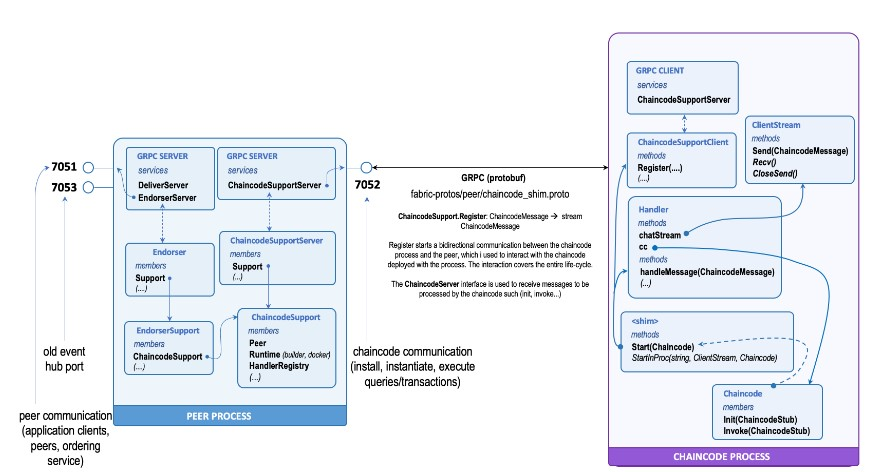
\includegraphics[width=\textwidth]{Images/peer_chaincode_interaction}
%\caption{}
%\label{fig:peerchaincodeinteraction}
%\end{figure}



\subsection*{Chaincode shim}

Con el fin de simplificar la vida del desarrollador y centrar sus esfuerzos en implementar la lógica del contrato inteligente, Hyperledger proporciona los \textit{chaincode shims}. Se trata de la implementación del \textit{runtime environment} necesario para integrar el contrato inteligente con Hyperledger Fabric y ejecutarlos como procesos remotos.

%El \textit{shim} es el componente responsable de ejecutar el contrato inteligente, hacerlo accesible para el nodo \textit{peer} y administrar toda la interacción de bajo nivel con él a través de gRPC. Además, proporciona una interfaz simplificada para el contrato inteligente para acceder a los servicios de invocación del \textit{ledger} y el \textit{chaincode} a través del \textit{chaincode stub} [\cite{hlf-internals}].

La figura \ref{fig:chaincodeshim} proporciona un desglose de los componentes que conforman el proceso chaincode junto con el rol y las responsabilidades que tiene cada uno de los componentes. Vale la pena señalar que, si bien el \textit{shim} es un componente específico del proceso chaincode, a menos que se especifique lo contrario, el \textit{shim} también se usa para referirse al conjunto de componentes que conforman el proceso chaincode, excepto por la implementación del contrato inteligente.

\begin{figure}[tbph]
\centering
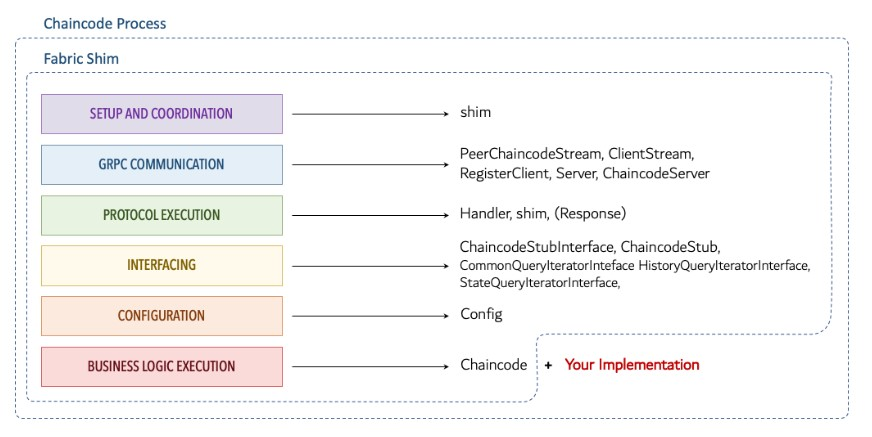
\includegraphics[width=\textwidth]{Images/chaincode_shim}
\caption{Componentes del chaincode shim}
\label{fig:chaincodeshim}
\end{figure}


\subsection*{Patrones de ejecución de Chaincode}

El \textit{shim} de Fabric admite dos modalidades de ejecución, que controlan el comportamiento de la conexión entre el \textit{chaincode} y el nodo \textit{peer}:

\begin{enumerate}
\item \textbf{Chaincode como cliente:} esta es la modalidad por defecto y la única utilizada en Hyperledger Fabric v1.4 [\cite{hlf-internals}]. Presenta el proceso chaincode como un cliente que inicia la conexión con el \textit{peer}.

\item \textbf{Chaincode como servidor:} A partir de la versión 2.0, Hyperledger Fabric admite la implementación de chaincode fuera de la blockchain [\cite{hlf-internals}]. De esta forma, el chaincode se ejecuta como un servidor independiente del \textit{peer}. En este escenario, no es necesario construir y lanzar el chaincode para cada \textit{peer}.
\end{enumerate}

\subsection*{Protocolo de interacción}
El protocolo de interacción se basa completamente en el intercambio de mensajes \textit{Protobuf} de tipo \texttt{ChaincodeMessage} entre el proceso chaincode y el \textit{peer}. La ventaja de usar \textit{Protobuf} es desacoplar la semántica de la implementación.

\begin{figure}[tbph]
\centering
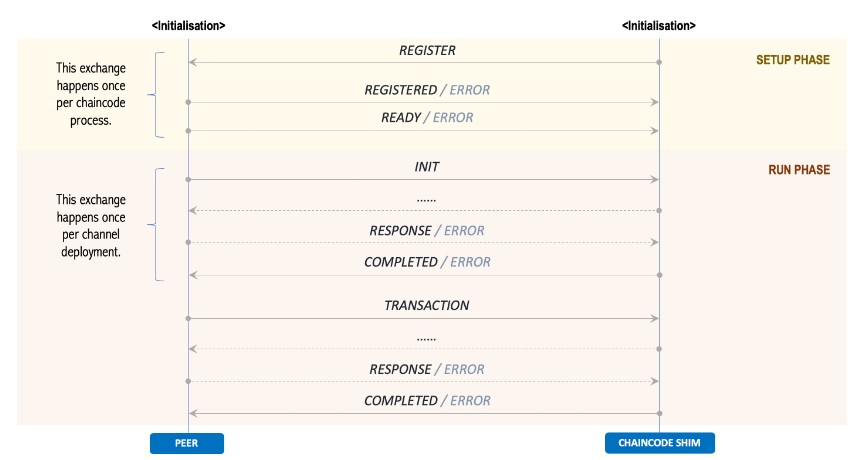
\includegraphics[width=\textwidth]{Images/interaction_protocol}
\caption{Interacción entre cliente y servidor gRPC}
\label{fig:interactionprotocol}
\end{figure}

La figura \ref{fig:interactionprotocol} proporciona una descripción general del protocolo de interacción de extremo a extremo. El ciclo de vida de la interacción se desarrolla en tres fases: inicialización, configuración y ejecución de la transacción (o fase de ejecución). En las siguientes secciones se proporcionarán más detalles para cada una de las fases.

\subsection*{Fase 1: Inicialización}
Durante la fase de inicialización, el \textit{peer} realiza una serie de operaciones:

\begin{enumerate}

\item Inicializa un objeto \texttt{ChaincodeSupport} que expone los servicios del \textit{chaincode} al nodo \textit{peer}.

\item Inicia un servidor gRPC de tipo \texttt{ChaincodeSupportServer} y registra el servicio \texttt{ChaincodeSupport} para habilitar la interacción con los procesos del \textit{chaincode}.

\item Inicia un servidor gRPC de tipo \texttt{EndorserServer}  para recibir propuestas de transacción para ser aprobadas.
\end{enumerate}

Por otro lado, el \textit{shim} carga el \textit{chaincode} invocando la función  \texttt{shim.Start(Chaincode)}, encargada de realizar las siguientes operaciones:

\begin{enumerate}
\item \textbf{Inicialización del cliente gRPC:} se utiliza para conectarse al \textit{peer} y configurar un flujo bidireccional para intercambiar instancias de \texttt{ChaincodeMessage}.

\item \textbf{Inicialización del \textit{handler}:} este componente se encarga de procesar todos los mensajes enviados por el \textit{peer} y ejecutar las operaciones asociadas.

\item \textbf{Inicialización del ciclo de procesamiento de mensajes:} este se utiliza para recibir los mensajes del \textit{peer} y enviarlos al \textit{handler} para su posterior procesamiento.
\end{enumerate}

Esta modalidad de inicialización admite el patrón \textbf{chaincode como  cliente}, donde el proceso \textit{chaincode} es un cliente para el \textit{peer}. El \textit{shim} también tiene la capacidad de inicializarse para admitir el patrón \textbf{chaincode como servidor}, donde los roles se invierten.

\subsection*{Fase 2: Configuración}
Antes de iniciar el ciclo para recibir de mensajes, el \textit{shim} envía un mensaje \texttt{REGISTER} a través del flujo bidireccional abierto con el \textit{peer}. Este mensaje contiene los detalles del \textit{chaincode} para registrarse codificado como \texttt{ChaincodeID}.
Al recibir el mensaje, el \textit{peer} valida la información asociada al \textit{chaincode} y crea una instancia de \textit{Handler} para manejar el intercambio de mensajes con el proceso del \textit{chaincode}. Luego, el \textit{peer} responde con un mensaje \texttt{REGISTERED} e inmediatamente después con un mensaje \texttt{READY}, lo que indica la finalización del proceso de configuración.

\subsection*{Fase 3: Ejecución de la transacción}
Una vez que se completa la fase de configuración, el \textit{chaincode} y el \textit{peer} están listos para ejecutar transacciones.

%A partir de este punto, la interacción es impulsada por el peer, como resultado de las operaciones que envían los clientes de la aplicación al peer. Por lo general, implican el despliegue del chaincode en un canal específico y la posterior invocación de transacciones en el contrato inteligente implementado.

Esta interacción se implementa en los siguientes pasos:

\begin{enumerate}
\item Como resultado del despliegue del \textit{chaincode}, el \textit{peer} envía un mensaje \texttt{INIT}. 

%El \textit{handler} inicializa un contexto de transacción para la simulación de la propuesta de transacción asociada a la inicialización y envía el mensaje a través de un flujo bidireccional.

\item Tras la recepción del mensaje \texttt{INIT}, el \textit{handler} crea una nueva instancia de \textit{ChaincodeStub}, que representa la interfaz para los servicios expuestos al contrato inteligente. Luego se invoca \texttt{Chaincode.Init()} pasando el \textit{stub} como argumento.

\item El \textit{chaincode} ejecuta la inicialización del contrato inteligente y el método \texttt{Init()} se completa con éxito o con un error. El primero hace que se envíe un mensaje \texttt{COMPLETED} al \textit{peer}, mientras que el segundo provoca un mensaje de \texttt{ERROR}.

\item Al recibir el mensaje, el \textit{peer} invoca el método \texttt{Handler.Notify()} en la instancia asociada al \textit{chaincode}. Este método cierra el contexto de transacción previamente abierto y hace que el método \texttt{Handler.Execute()} desbloquee y devuelva la respuesta obtenida por el \textit{chaincode}.

\end{enumerate}

Las invocaciones posteriores del mismo \textit{chaincode} en el mismo canal dan como resultado que el \textit{peer} envíe un mensaje \texttt{TRANSACTION}, que se maneja de la misma manera que se detalla para el mensaje \texttt{INIT}.






